\chapter{Datasets}
High dimensional datasets are not a very common research topics. In this chapter I will describe some data sources and possible applications of the described algorithm. I also show some interpretations of subspaces in different datasets and some failed approaches of finding them. To get, isolate and preprocess the data I've used some scripts. Because I think open research should not only contain open publications but also open data sources, you can find the scripts and some notes about them online.\footnote{\url{https://github.com/crepererum/GSD}} Should you have some questions, find a bug or want to contribute, feel free to use the issue tracker or file a pull request.

\section{Drug Database}
Another source of high dimensional data is the list of incredients of drugs. A given set of drugs described by a list of their incredients is processed as followed: Build a list of all incredients in all drugs and bring them into a fixed order. Every incredient forms one dimension. Then build a binary vector for every drug in the database where $1$ describes that a incredient is contained in the drug and $0$ if this is not the case.
\begin{figure}
	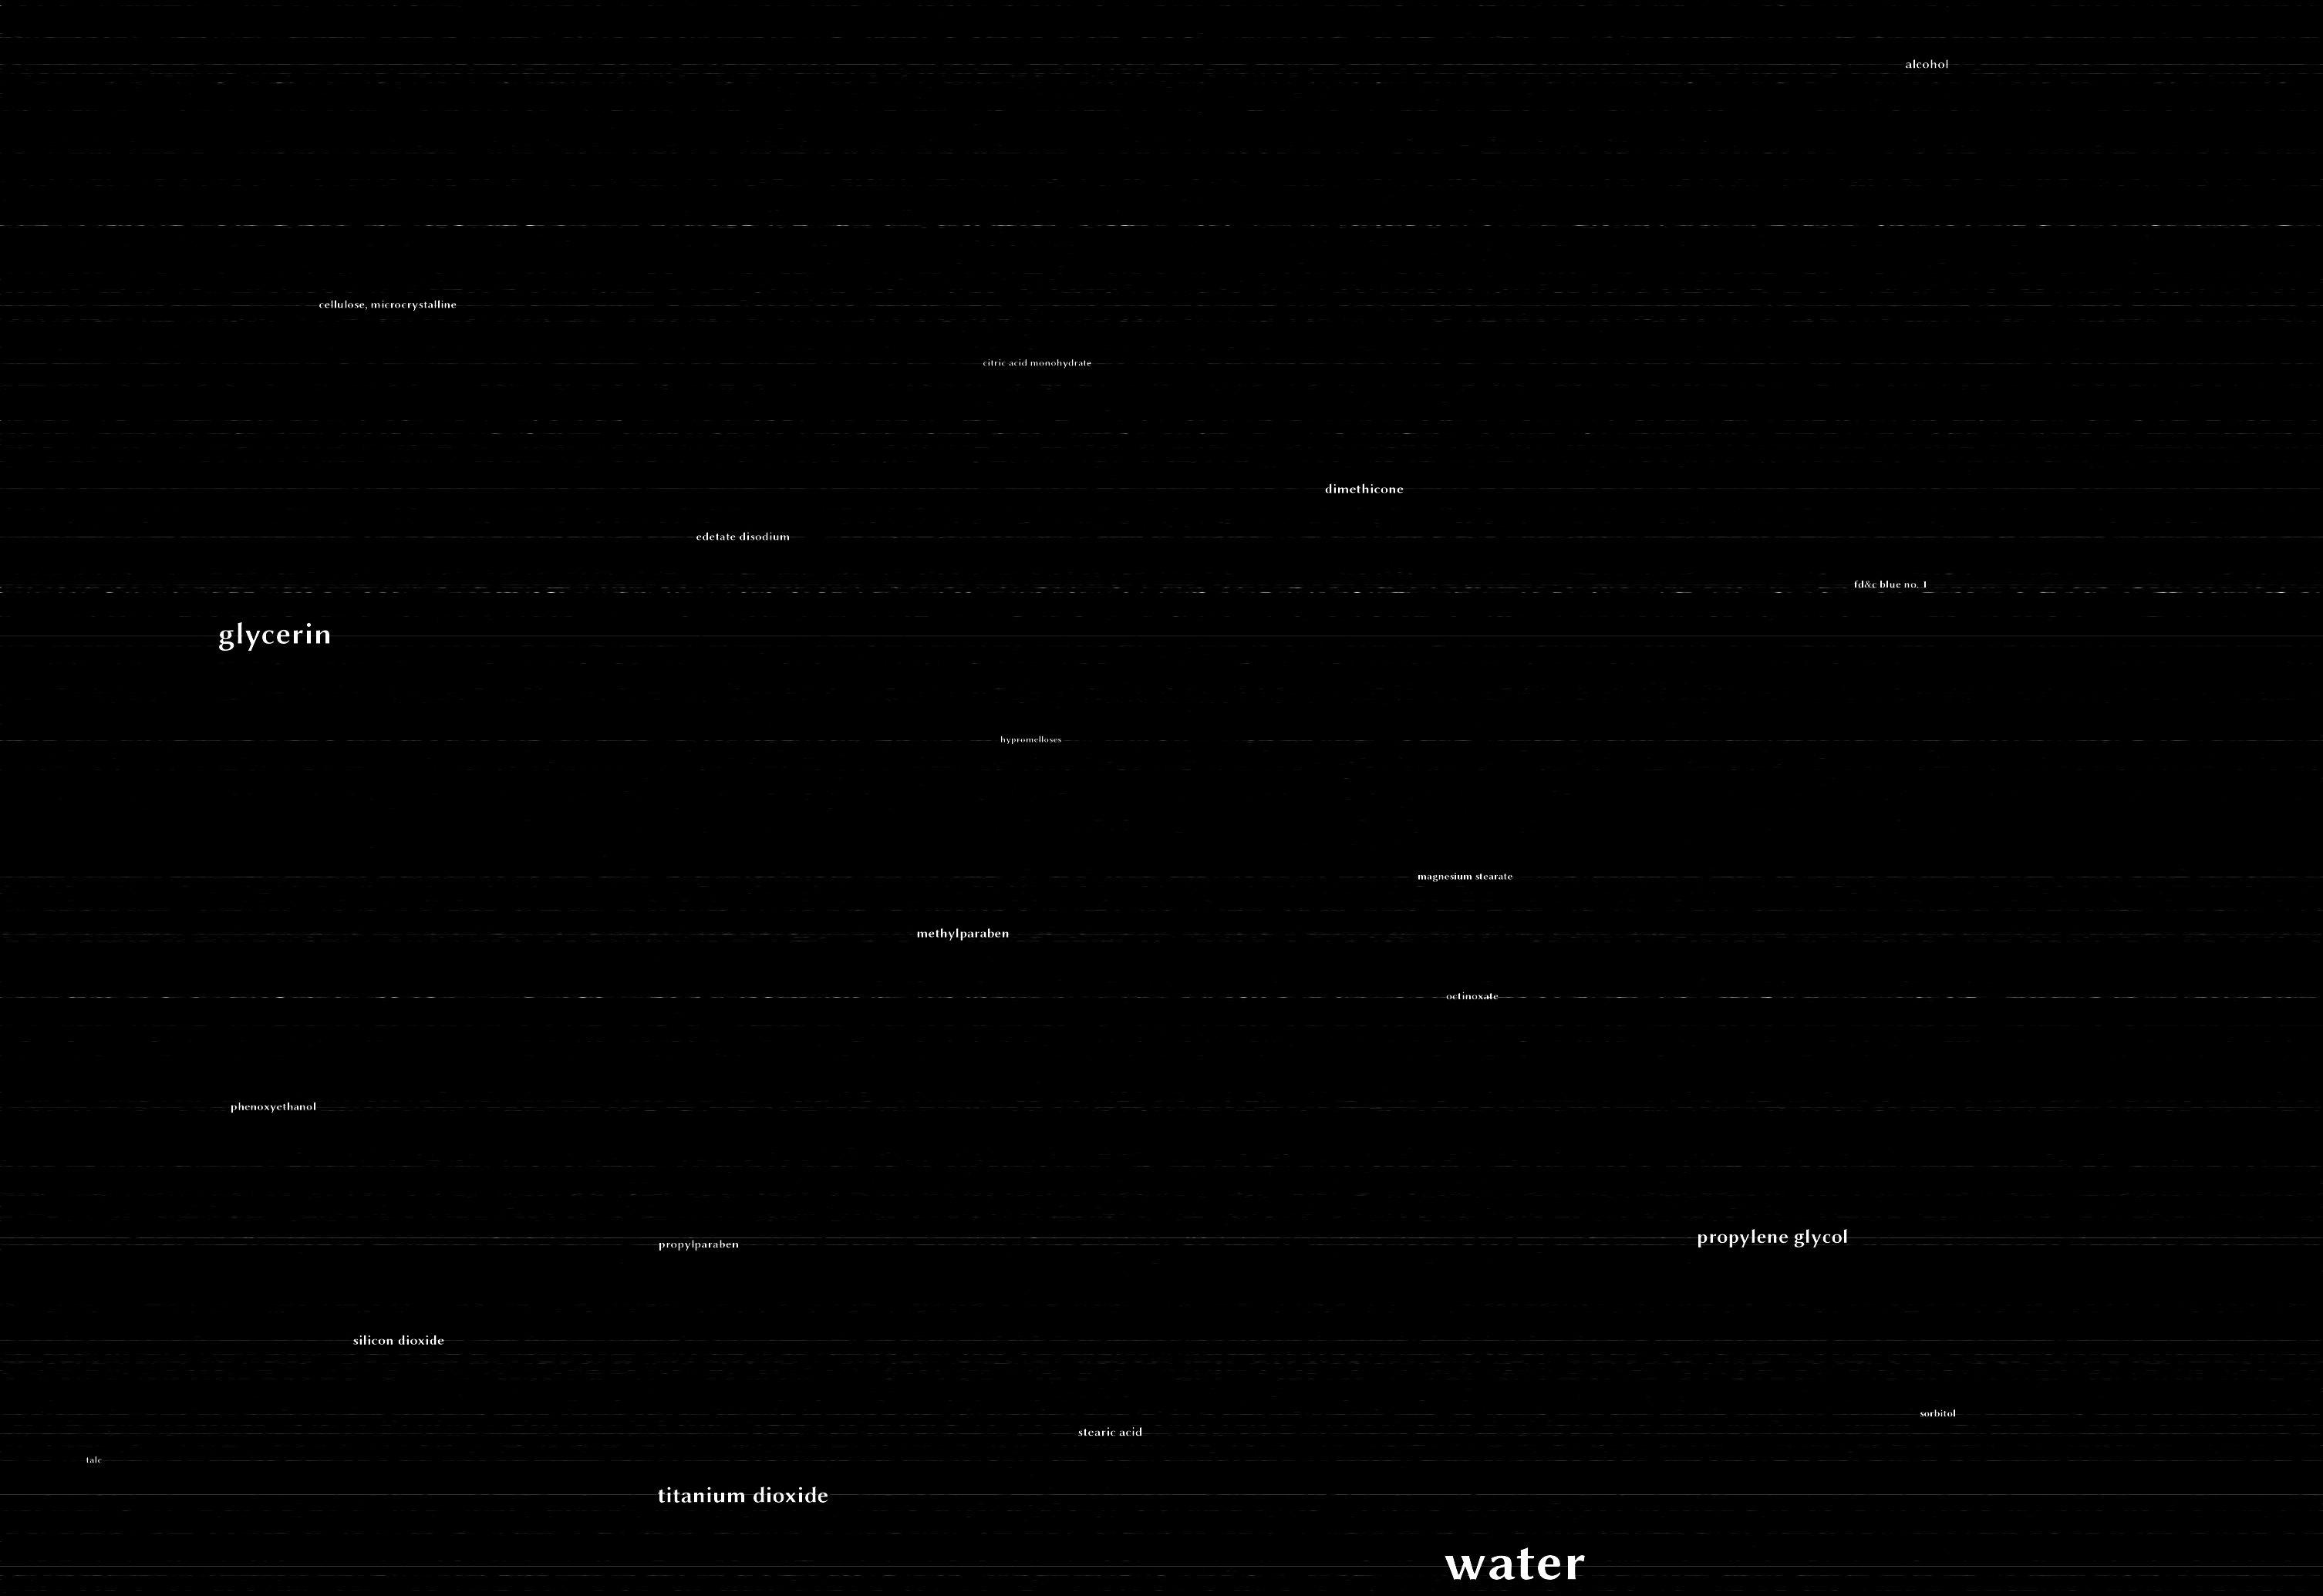
\includegraphics[width=\textwidth,keepaspectratio]{drugs}
	\caption{drugs spectrum}
	\label{fig:drugs}
\end{figure}
I hoped to find some public drug data bases containing drugs registered in Germany or in the EU. But this was not the case. Either they were only usable via a very limited interface or it would cost me a enorm amount of money to buy a license. Since the open data movement in USA has a very long tradition, it was easy to find an american drug database, that is easy to parse and provides a huge data collection.\footnote{\url{http://dailymed.nlm.nih.gov/dailymed/downloadLabels.cfm}} I provide a parser and converter for this kind of data.

